\scanpage{104}
\mspage{51}
which are induced by the normalization morphisms between m.graphs associated with the \unsure{one|one}-point graphs. Of course, to be able actually to reconstruct the \inserted{effects \deleted{\unsure{the interaction}} on $\Pi_1M$ of the} normalization morphisms, and their commutation properties with isomorphisms, one must use the \deleted{\unsure{covariances|commutations}} commutation of (148) with
\[
\unsure{\mathfrak S|\mathcal G}_{I,I'}\simeq\unsure{\mathfrak S|\mathcal G}_{I'}\times\unsure{\mathfrak S|\mathcal G}_{I\setminus I'}\qquad\ldots
\]

\uline{Program} Determine (up to ``canonical'' equivalence) all the groupoids $\Pi_1M_{g,I}$, with their functorial dependence for \inserted{fixed $g$,} variable $I$ (monomorphisms $I'\hookrightarrow I$) via the normalization morphisms (148).
\margin{by ``generators and relations'' — \unsure{defined|defined|define} in purely algebraic terms\ldots}

Moreover, for every MD-graph $G$, determine the extension $S\Pi_1M_G$ of
\[
\Pi_1M_G\simeq\prod_{\alpha\in S(G)}\Pi_1M_{\alpha,\widehat I_\alpha}\quad\text{by }\mathbb Z^{\widetilde A(G)},
\]
and for a generization morphism (for example an isomorphism!) \deleted{\unsure{given}} $G\longrightarrow G'$ of MD-graphs, \deleted{\unsure{define}}\inserted{determine} the corresponding generization morphism of groupoids
\[
S\Pi_1M_G\unsure{\longrightarrow|\rightharpoondown}S\Pi_1M_{G'}.
\]
\margin{\figure{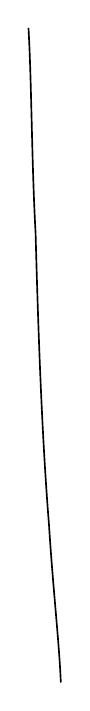
\begin{tikzpicture}[x=1cm,y=1cm]
\draw[line width=0.6pt,line cap=round] (0,0) .. controls (0.04,-0.7) and (0.04,-1.7) .. (0.09,-2.6) .. controls (0.13,-4.1) and (0.18,-5.3) .. (0.26,-6.3) .. controls (0.31,-7.1) and (0.39,-7.8) .. (0.41,-8.3);
\end{tikzpicture}}}
\margin{1\unsure{0|9}3}
